%\documentclass{ExcelAtFIT}
%\documentclass[czech]{ExcelAtFIT} % when writing in CZECH
\documentclass[slovak]{ExcelAtFIT} % when writing in SLOVAK


%--------------------------------------------------------
%--------------------------------------------------------
%	REVIEW vs. FINAL VERSION
%--------------------------------------------------------

%   LEAVE this line commented out for the REVIEW VERSIONS
%   UNCOMMENT this line to get the FINAL VERSION
%\ExcelFinalCopy


%--------------------------------------------------------
%--------------------------------------------------------
%	PDF CUSTOMIZATION
%--------------------------------------------------------

\hypersetup{
	pdftitle={Paper Title},
	pdfauthor={Author},
	pdfkeywords={Keyword1, Keyword2, Keyword3}
}


%--------------------------------------------------------
%--------------------------------------------------------
%	ARTICLE INFORMATION
%--------------------------------------------------------

\ExcelYear{2017}

\PaperTitle{Simulátor šírenia radarového signálu}

\Authors{Michal Ormoš*}
\affiliation{*%
  \href{mailto:xormos00@stud..vutbr.cz}{xormos00@stud..vutbr.cz},
  \textit{Fakulta informačních Technologií, Vysoké učení technické v Brně}}
%%%%--------------------------------------------------------
%%%% in case there are multiple authors, use the following fragment instead
%%%%--------------------------------------------------------
%\Authors{Jindřich Novák*, Janča Dvořáková**}
%\affiliation{*%
%  \href{mailto:xnovak00@stud.fit.vutbr.cz}{xnovak00@stud.fit.vutbr.cz},
%  \textit{Faculty of Information Technology, Brno University of Technology}}
%\affiliation{**%
%  \href{mailto:xdvora00@stud.fit.vutbr.cz}{xdvora00@stud.fit.vutbr.cz},
%  \textit{Faculty of Information Technology, Brno University of Technology}}

\Keywords{Radar --- Simulácia --- Matlab}

\Supplementary{\href{http://youtu.be/S3msCdn3fNM}{Demonstration Video} --- \href{http://excel.fit.vutbr.cz/}{Downloadable Code}}


%--------------------------------------------------------
%--------------------------------------------------------
%	ABSTRACT and TEASER
%--------------------------------------------------------



\Abstract{
Táto správa je predmetom Bakalárskej práce, ktoá vznikla na Fakulte Informačných Technológií v Brne a pojednáva o Simulátore širenia radarového signálu. Cieľom, ako názov napovedá bolo vytvoriť simulátor, ktorý by bol schopný v abstraktnom prostredí simulovať celý priebeh zachytávania signálu vyslaného z radaru, cez odrazenie od objektu až po prijatie vracajucého sa signálu spať do radaru.
Problém bol riešený v prostredí Matlab a to simuláciou trojrozmerného priestoru, ktorý obsahuje rôzne body, statické aj dynamické, ktoré reprezentujú radar a objekty ktoré sleduje. V rámci tohto prostredia sa počítajú, získavajú a spracuvávajú všetky potrebné dáta od vzdialeností, uhlov až po výpočty frekvencie a výkonu vracajucého sa signálu.
Výsledkom celej práce je plnohodnotne nasimulované prostredie, ktoré demonštruje celý proces zahytenia objektu radarom a následne jeho zobrazenie v sprektograme, ktorý odráža rýchlosť objektu voči radaru.
Využitie tohto simulátora je vhodné pre všetky vedecké skupiny, ktoré sa zaujímajú o radarové technológie a spracovávanie výsledkov z ich výstupov. Moja technológia by im mohla ušetriť drahocený čas a snahu v montovaní reálných setup-ov v teréne a získaváni vysledkov. Teda by mohli pohodlne testovať roôzne setup-y a konfigurácie z pohodlia domova. Rovnako by mohla byť práca použitá ako vyučovacia pomôcka pre lepšie pohopenia činnosti radaru.
}

% \Teaser{
% 	\TeaserImage{placeholder.pdf}
% 	\TeaserImage{placeholder.pdf}
% 	\TeaserImage{placeholder.pdf}
% }



%--------------------------------------------------------
%--------------------------------------------------------
%--------------------------------------------------------
%--------------------------------------------------------
\begin{document}

\startdocument


%--------------------------------------------------------
%--------------------------------------------------------
%	ARTICLE CONTENTS
%--------------------------------------------------------

%--------------------------------------------------------
%--------------------------------------------------------
%--------------------------------------------------------
%--------------------------------------------------------
\section{Úvod}
\label{sec:Intorduction}
\hspace{0.6cm}\textbf{Motiváciou} pre vznik tohto projektu bol možný prinos k výzkummnej skupine na Fakulte Informačných technológií v Brně zaoberajúcej sa technolǵiou využitia radarov. Takýto druh softwaru nemajú k dispozícií a nič podobného charakteru vo svete softwaru ešte nenašli.

\textbf{Definícia problému} je, že potrebujeme simulovať radar ako technológiu a to presne šírenie jeho okom neivditiľného singálu, ktorý sa presúva v priestore. Tento signál sa môže od niektorých objektov v dohľadnej vzdialenosti odraziť a vrátiť spať do radaru. S informáciou o výkone vyslaného signálu a prijatého signálu sme schopný zisťit napríklad rýchlosť, vzdialenosť, orientáciu pohuby či typ objektu aký pred radarom stojí alebo stál.
Využitie radaru si vie každy živo predstaviť v policajných radaroch, námorníctve či letectve.
My sme sa zamerali na obecne použivané radary značky od firmy RFBeam, ktoré využívajú pracovníci fekulty.

\textbf{[Existing solutions]} 

\textbf{[Our solution]}

Možný \textbf{príspevok} pre vedu a výzkum je veľmi jasný. Výzkumné skupiny by túto technológiu mohli využivať pri svojej práci, čo by im ušetrilo energiu a snahu v manuálnom budovaní setupov a získavaní dát, ktoré by ďalej použivali na spracovanie sinálov. Rovnako by tento modul mohol slúžiť ako výukový prostriedok pre lepšie pochopenie a názornú ukážku prace radaru v interaktívnym spôsobom zmeny prostredia, čo by vyústilo k rôznym výsledkom, ktoré pomôžu študentovi lepšie pochopiť význam a použitie technológie.

%--------------------------------------------------------
%--------------------------------------------------------
%--------------------------------------------------------
%--------------------------------------------------------
\section{Radar}
\label{sec:Radar}
	\hspace{0.6cm}Radar (skratka anglického slova \textbf{RA}dio \textbf{D}irection \textbf{A}nd \textbf{R}anging) je elektromagnetický senzor pre detekciu a lokáciu objektov. Jeho všeobecný princíp fungovania môže byť zhrnutý v  nasledujúcich bodoch \cite{radartutor}\cite{radarhandbook}:
	\begin{itemize}
	\item Radar vysiela zo svojej antény elektromagnetické vlny, ktoré sa šíria priestorom v určitom smere.
	\item Niektoré z vysielaných vĺn sú zachytené objektami, ktoré tento signál pohlcujú a odrážajú, nazývame ich ciele radaru a väčšinou sú v určitej vzdialenosti od radaru.
	\item Časť tejto energie, je pohltená cieľovým objektom, zvyšok je odrazený naspäť mnohými smermi.
	\item Niektoré vlny z tejto spätne vysielanej energie sa vrátia naspäť k radaru a sú zachytené radarovým príjmačom umiestnenom na anténe.
	\item Po zachytení signálu, sú tieto dáta vhodne spracované a analyzované. Vo výsledku zistíme či su získané informácie naozaj požadované dáta z odrazeného cieľového objektu.
	\end{itemize}

	\textbf{Základné časti radaru}
    \begin{enumerate}
      \item \textbf{Anténa} Je to čo spája radar s vonkajším svetom. Vykonáva viac funkcií: \begin{itemize}
      		\item Dovoľuje šíriť vysielanú energiu z vysielača.
      		\item Zhromažduje zachytenú energiu odrazenú z cieľa pre príjmač.
      		\item Poskytuje informáciu o azimute a elevácii radaru k cieľu.
      		\item Jej tvar, veľkosť a funkčnosť určuje skúmaný objem priestoru
      	\end{itemize}
      \item \textbf{Vysielač} Dôležitá časť radaru, ktorá generuje a vysiela signál v požadovanej vlnovej dĺžke, Signál je generovaný zo zdroja (\textbf{generátor signálu}), potrebný výkon sa získava použitím výkonneho oscilátora alebo zosilňovača spolu s nízkonapätovým zdrojom. 	
      \item \textbf{Príjmač} Zachytavá prijatú odrazenú energiu z cieľa. Vzhľadom na vzdialenosť a materiál objektu od ktorého bol signál odrazený sa bude odvíjat jeho intenzita, ktorá dosahuje veľmi malé hodnoty (väčšinou až $10^{-9}$W). Preto sa signál musí zosíliť pomocou \textbf{Zosilovača} pre dalšie spracovanie a je doležité aby anténa neobsahovala žiaden šum. Nasleduje \textbf{mixér}, ktorý porovnám referenčný signál z \textbf{oscilátora} s prijatým signálom. Potom sa môže začať časť spracovania a extrakcie informácii zo signálu. Pomocou zosilovačov a filtrov pre spracovanie signálov.
      \item \textbf{Prepínač} Prvok slúžiaci k tomu aby sa prepínala funkcia prepínača a vysielača na anténe. Touto zmenou funkcie chráni citlivé zariadenie príjmača popritom ako vysielač vysiela. Rovnako presmerúva šum vysielača do príjmača, ktorý ho môže dopredu vyfiltrovať.
      \item \textbf{Zosilňovač} V prípade vysielania signálu je jeho úlohou zosíliť signál pred vyslaním, aby sa napriek jeho diaľke, ktorú musí k cieľu uraziť vrátil čo najintenzívnejší. V prípade príjmania signálu ho taktiež zosilňuje, pretože vracajúci sa signál ja veľmi malý.    
    \end{enumerate}

    Radar K-MC4 od Švajčiarskej spoločnosti RFBeam Microwave GmBH je pre nás implicitný radar a budeme to v tejto práci simulovať.

%--------------------------------------------------------
%--------------------------------------------------------
%--------------------------------------------------------
%--------------------------------------------------------
\section{Simuláčné prostredie}
  \textbf{Radar v priestore}\\
    \hspace{0.6cm}V návrhu simulačného prostredia si pre jednoduchosť vysvetlenia predstavme kocku, ktorá tvorí náš priestor pre umiestnenie radaru, objektu a definovanie podmienok, ktoré pre simuláciu radaru potrebujeme. Ako scénu si predstavme meranie rýchlosti na diaľnici s použitím radaru umiestnenom na vyvýšenou mieste, ktorý sleduje vozidlá na vozovke pod ním.

    V priestore je teda umiestnený radar, pre predstavu napríklad na dialničnom moste, ktorého zorné pole smeruje na diaľnicu pod nim, teda objekty, ktoré radar sleduje ho míňajú po jeho vertikálnej ose, teda prechádzajú pod ním.
    % Táto predstava je základná a postavenia sa budú dať meniť. 

	\begin{figure}[t]
		\centering
		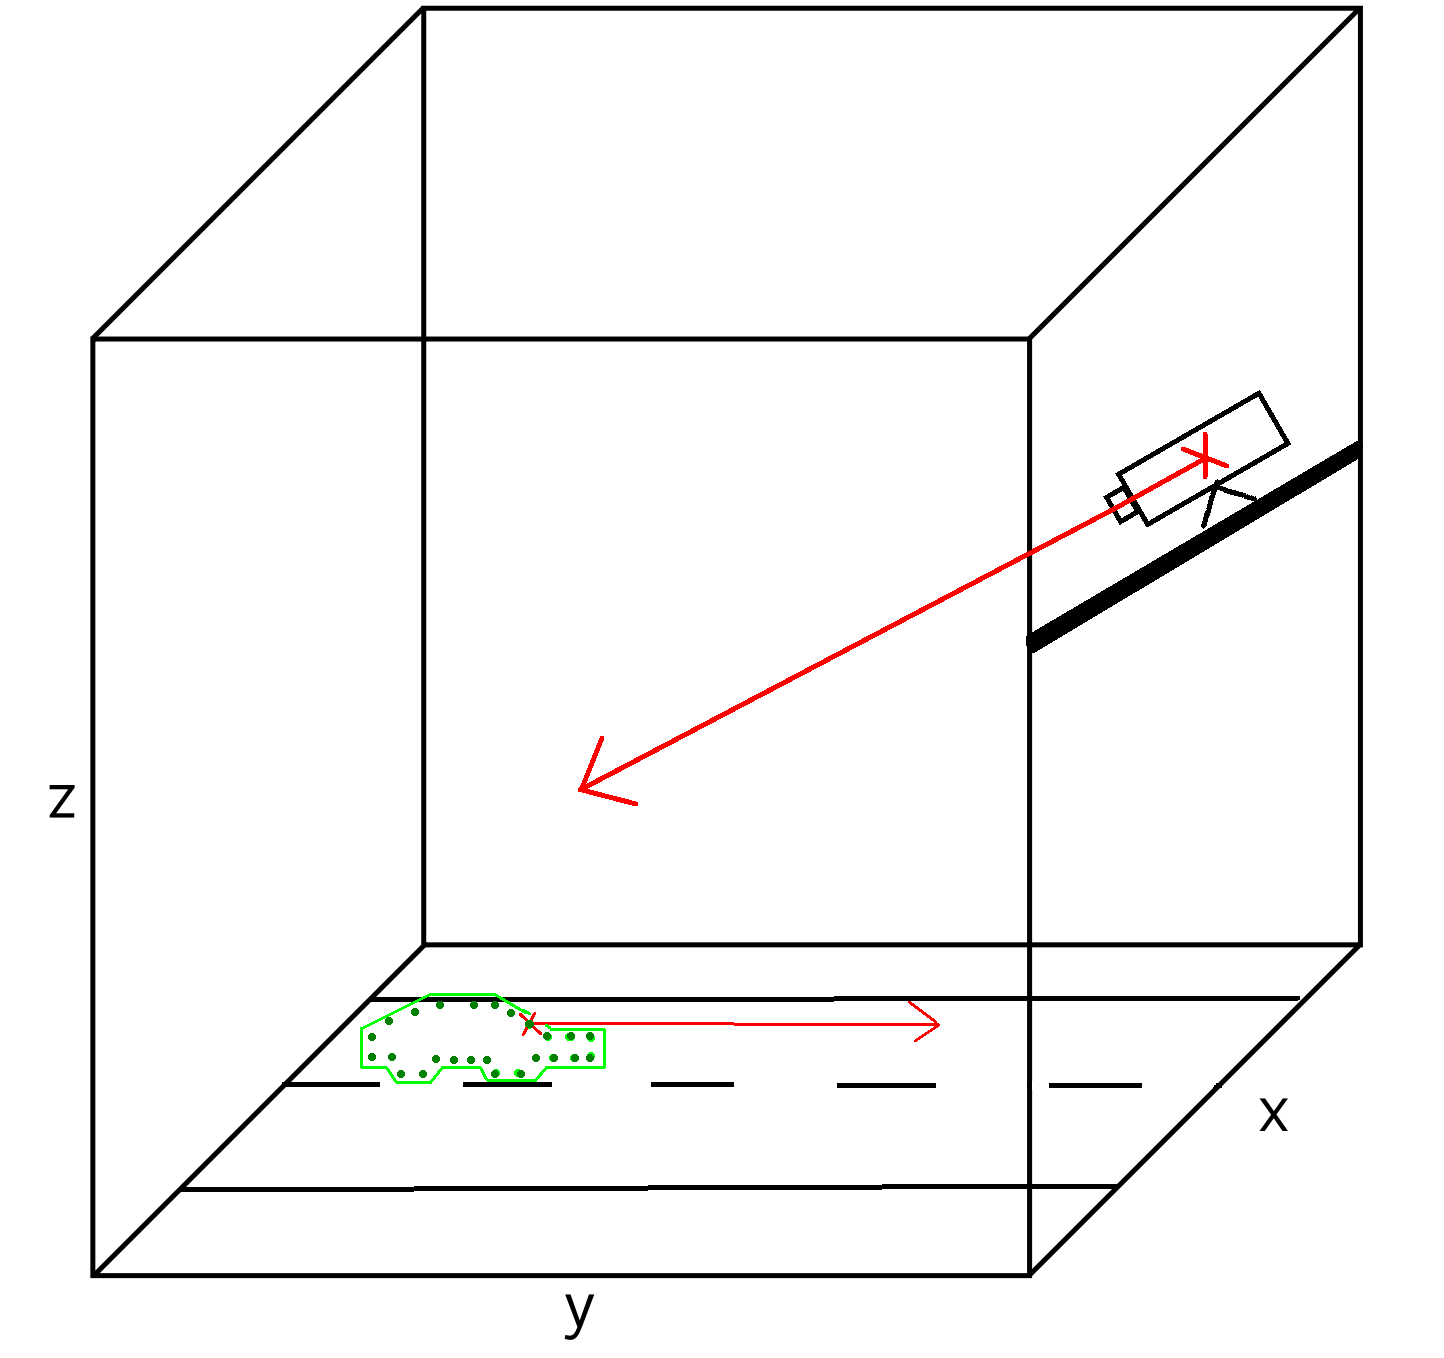
\includegraphics[width=1.0\linewidth]{cube_radar_car.png}
		\caption{Základná predstava priesotru, ktorý budeme simulovať.}
		\label{fig:cube_radar_car}
	\end{figure}

    Radar bude reprezentovaný ako práve jeden nehybný bod v priestore. Tento bod má mať presne určéne svoje súradnice v priestore, ktoré charakterizujú jeho polohu. Rovnako obsahuje vektor, ktorý určuje bod kam radar mieri. To znamená, že je nevyhnutne dôležité vedieť kam radar presne mieri počas celej simulácie. Radar bude možné jednoducho natáčať po vertikálnej a horizontálnej ose pomocou jeho vektoru. Voliteľne môžeme pridať aj naklonenie radaru na mieste, do strán \ref{fig:cube_radar_car}.
    
    Bod definujúci polohu radaru bude slúžiť ako miesto pre generovanie signálu a zdroj vysielania paprskov na vektor zorného poľa radaru. Podľa súradníc polohy radaru a vektoru radaru sme schopný určiť nevyhnutné uhly a vzdialenosti, ktoré budeme potrebovať pre výpočty simulácie.

  \textbf{Objekt v priestore}\\
    \hspace{0.6cm}Pre správnu funkciu radaru a získanie čo najväčšieho množstva simulačných dát je potrebné rovnako ako aj v návrhu samotného radaru, aj čo najpresnejšie popísať objekt na ktorý budeme v simulácii vysielať naše paprsky, teda cieľ radaru. 

    Objekt preto budeme reprezentovať ako zhluk bodov v určitom tvare, ktorý pripomína objekt reálneho sveta, ako napriklad v našom návrhu, osobné vozidlo.

    Každý tento bod objektu, pričom počet bodov ohraničujúci objekt bude vopred určený, bude pre radar vnímaný ako samostatný objekt a bude obsahovať svoje súradnice v priestore.
    Každý tento bod, ktorý je vlastne objekt bude vykonávať pohyb v priestore, čo bude reprezentovať pohyb celého objektu. Tento pohyb bude reprezentovaný vektorom pohybu bodu, čo je vlastne vektor, ktorý obsahuje aktuálne súradnice bodu vo vzťahu so súradnicami bodu v ďalšom časovom okamžiku . Súčasťou jeho pohybu bude aj rýchlosť pohybu objektu, ktorá bude dopredu definovaná a potrebná pre dalšie výpočty. Všetky body v objekte sa teda budú zdanlivo pohybovať ako jeden celok \ref{fig:cube_radar_car}.

    Podstatnou charakteristikou bodu bude jeho RCS (Radar Cross-section), ktorý reprezentuje ako intenzívne bude daný bod reagovať na prijatý signál, teda akou silou a smerom odrazi signál näspať. To všetko závisí na simulovanom tvare a materiálu objektu, rovnako ako aj uhlom pod akým je voči paprsku. RCS sa bude dať jednoducho nastaviť ako vstupná hodnota programu. Rovnako ako súradnice umiestnenia bodov, rýchlosť objektu a...

	Radar KMC-4, ktorý sme sa rozhodli pre túto simuláciu používať ako referenčný má svoje vlastnosti, ktoré musíme implementovať aj do našeho simuláčného radaru. Všetky tieto údaje boli predom získane vyrobcom tohto radaru, firmou RFbeam a sú umiestnené v jeho datasheete \cite{kmc4sheet}, preto ich nemusíme nadobudnúť experimantálne.

  \begin{itemize}
    \item Vysielacia frekvencia radaru KMC-4 je 24.150GHz
    \item Zisk antény je 13dB
    \item Zisk vysielača
    \item Zisk príjmača
  \end{itemize}  

  \section{Charakteristika antény}
    Hardware samotného radaru mieri na určitý bod. Nemôže vysielať a príjmať všetky svoje paprsky do všetkých bodov a smerov rovnomerne. Charakteristika antény, resp. anténový diagram reprezentuje aké je potlačenie vysielaného signálu v decibeloch, jednotlivo v horizontálnom a vertikálnom smere vzhľadom na vysielaní signálu od vektoru radaru v uhlových stupňoch. Tento údaj je obsiahnutý v datasheete a je len graficky znázornený.

	\begin{figure}[t]
		\centering
		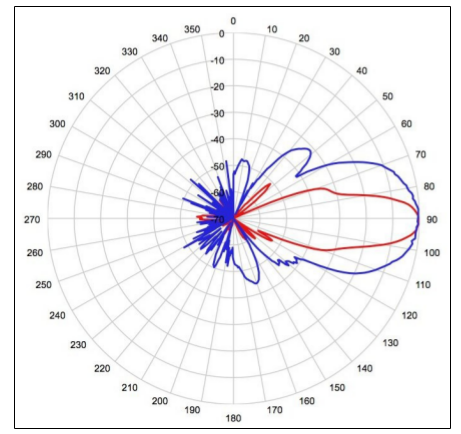
\includegraphics[width=1.0\linewidth]{kmc4_antenna_char.png}
		\caption{Diagram graficky zobrazujúci charakteristiku antény. Ktorý sme použili ako zdroj pre našu textovú verziu charakteristiky antény\cite{kmc4sheet}.}
		\label{fig:kmc4_antenna_char}
	\end{figure}

    Preto je potrebné extrahovať tento útlm antény pre každý stupeň jednotlivo. Pre tento prípad sme použili jednoduchú metódu za pomoci programu Gimp a jeho nástroja pre zmeranie uhlu a to nasledovne. Umiestnili sme jeden koniec pravítka do stredu obrázku a druhý koniec po čiare doprava vedúcej k uhlu 90 stupňov. Tento nástroj ďalej fungoval ako uhlomer a s uhlom v strede obrázku sme pohodlne vyčitali pre každý červený (horizontálny) a modrý (vertikálny) bod jeho útlm v určitom uhle \ref{fig:kmc4_antenna_char}.

    Celý tento proces sa zapisoval do súboru vo formáte .csv. Jeden súbor obsahuje informácie v rozsahu $0^{\circ}-180^{\circ}$, delených po jednom stupni. Pre vertikálny smer a druhý súbor v rovnakom rozsahu pre horizontálny smer.

    180 získaných hodnôt pre nás avšak nebude dostačných. Nato aby sme signál rekenštruovali musíme dodržat Nyquistov teorém a predpokladaná frekvencia simulácie bude 10 kH. To nám spôsobí, že nami získané hodnoty su vo veľmi malom rozsahu a výsledný graf by bol zkockovatelý. Preto musíme tieto hodnoty interpolovať.

    Pôvodný interval hodnôt obsahuje $180$ bodov, ten vynásobime tísickou a pre týchto $180 000$ bodov sa malý interval interpoluje do veľkého pomocou matematickej metódy spline. To znamená, že pre väčší internal sme našli približné hodnoty funkcie medzi bodmi v danom menšom intervaly.

    Nami získaný a spracovaný útlm potrebuje pre využitie správny uhol, pre ktorý sa bude určovať. Ten musíme získat v našom trojrozmernom priestore jednotlivo pre horizontálnu a vertikálnu zložku dvojrozmerného priestoru.
    \newline

	\begin{figure}[t]
		\centering
		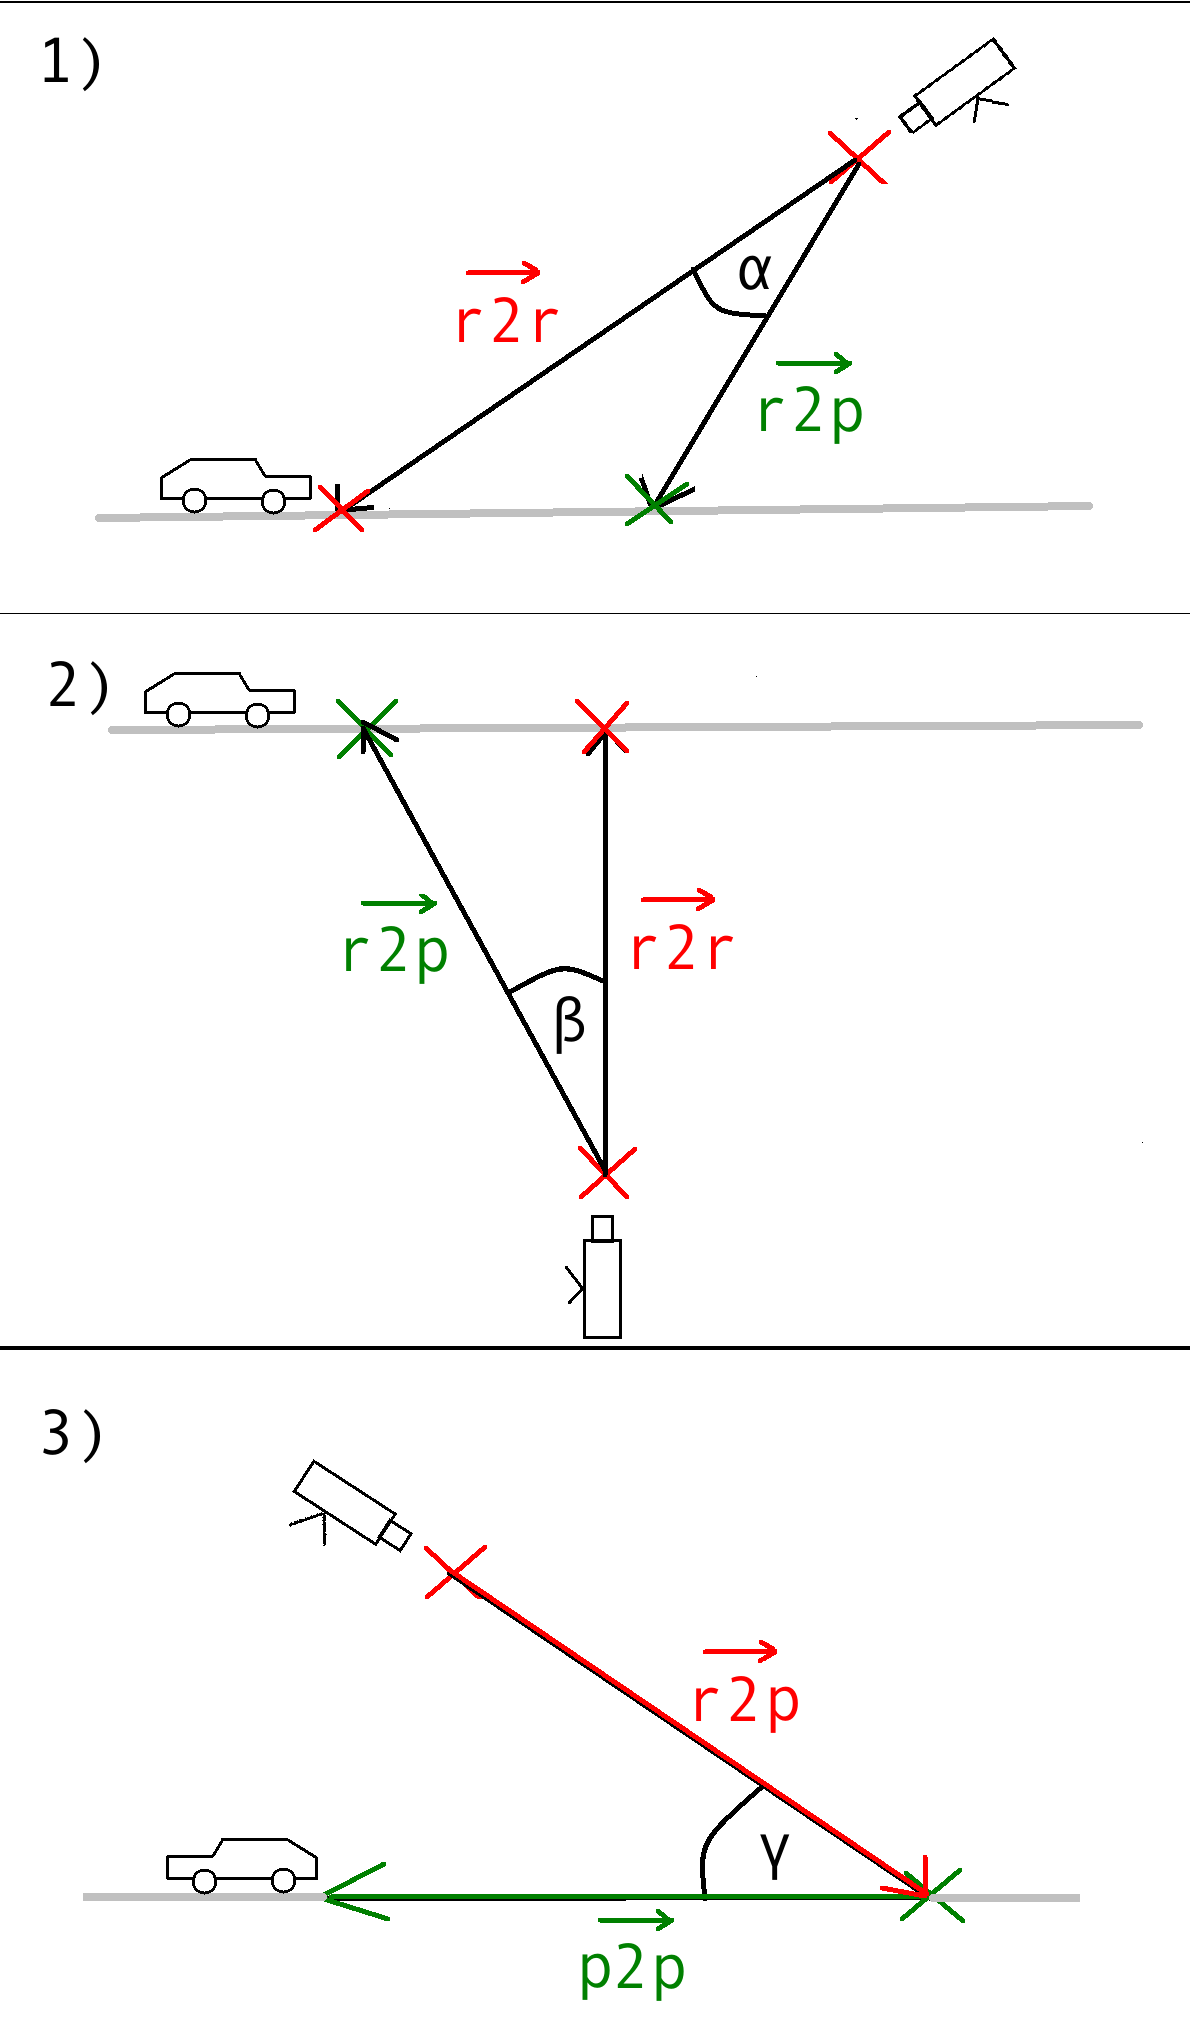
\includegraphics[width=1.0\linewidth]{radar_angles.png}
		\caption{Grafické znázornenie nami riešených a reprezenrtovaných uhlov. 1) Vertikálny 2) Horizontálny 3) Priestorový.}
		\label{fig:radar_angles}
	\end{figure}

    \textbf{Vertikálny uhol}

      Pomocou obrázku \ref{fig:radar_angles} čast 1) vidíme myšlienku pri získavaní hodnoty vertikálneho uhlu. Trojrozmerný priestor si premietnene do dvojrozmerného, teda vynecháme jeho x-ovú zložku.
      Poznáme vektor radaru, teda bod v ktorom sa radar nachádza a bod na ktorý mieri, označme si ho ako $\overrightarrow{r2r}$(radar to radar).
      Rovnako poznáme aj aktuálnu pozíciu objektu. Teda vieme určiť vektor od umiestnenia radaru k aktuálnej pozícii objektu v priestore, označme si ho ako $\overrightarrow{r2p}$(radar to point).
      Ziskaný uhol medzi vektormi $\overrightarrow{r2r}$ a $\overrightarrow{r2p}$, je náš žiadúci vertikálny uhol. 

    \textbf{Horizontálny uhol}

      Obdobne ako sme zíkali uhol vertikálny vieme získať aj uhol horizontálny, \ref{fig:radar_angles} čast 2). V tomto prípade pri premietnutí do dvojrozmerného priestoru vynecháme osu $z$, z troj rozmerného priesotoru.
      Rovnako využijeme vektory $\overrightarrow{r2r}$, $\overrightarrow{r2p}$ a získame požadovaný horizontálny uhol.
    \newline

    Pre uhlol vertikálny a horizontálny teraz vieme v každom okamžiku simulácie získať uhol radaru voči objektu. Tento uhol použijeme v nami predom pripravených .csv dátach a tým a získame stratu signálu v dB, osobitne pre horizontálny a vertikálny smer v danom časovom okamžiku a usporiadaní objektov priestore. Následne tieto 2 hodnoty vertikálneho a horizontálneho smeru medzi sebou vynásobíme a dostaneme aktuálnu stratu signálu v dB, pre náš bod v priestore voči radaru v danom časovom okamžiku. 
  
  \section{Vysielanie paprsku}
    \hspace{0.6cm}Ďalej pracujeme s predstavou nášho priestoru, našej kocky, v ktorej je umiestnený náš radar so svojimi súradnicami rovnako ako aj jeho bod, ktorého pohyb pozoruje. Medzi týmito dvoma bodmi nám vzniká vektor, teda to ako radar mieri na fiktívnu cestu pod ním.

    Z jednej strany kocky na druhú stranu sa nám pohybuje náš objekt, v tomto prípade osobné vozidlo, ktoré je reprezentovaný zhlukom svojich bodov. Každý bod ma rovnakú rýchlosť v a smer pohybu, ktorý určuje jeho vektor pohybu.

    Náš radar imaginárne vysiela nepretržite v každom okamihu pohybu objektu paprsok, čo v našej simulácií znamená veľa výpočtov pre charakteristika tohto imaginárneho paprsku.
    \newline

    \textbf{Vzdialenosť}

      Vzdialenosť objektu od radaru je potrebné pre výpočet vracajúcej sa energie do radaru, ktorú získame z radarovej rovnice.
      V našom simulačnom prostredí pre získanie hodnoty vzdialenosti využijeme Euklidovu vzdialenosť, čo je metrika daná dvoma vektormi umiestnenými v priestore.
      \newline

    \textbf{Priestorový uhol}

      Pre výpočet frekvencie signálu vracajucého sa do radaru budeme potrebovať priestorový uhol, ktorý zviera vektor radaru s vektorom pohybu objektu. \ref{fig:radar_angles} časti 3).
      Vektor radaru je nám už dobre známy a máme ho označený ako $\overrightarrow{r2r}$. Vektor pohybu objektu nie je nič iné ako jeho aktuálna pozícia v priestore vo vzťahu s jeho pozíciou v priestore v dalšom časovom okamzžiku, označme si ho $\overrightarrow{p2p}$ (point to point).
      Uhol, ktorý tieto 2 vektory zvierajú, je náš požadovaný priestorový uhol.
      \newline


    \textbf{Prijatý signál}

      Po správnom získaní priestorového uhlu, ktorý zviera vektor radaru s verktorom pohybu objektu, sme schopný v každom okamžiku pohybu objektu získať veľkosť sígnalu vracajucého sa od objekt späť do radaru a to pomocou vzťahu:

      \begin{equation} %\label{eq:0}
        F_{r} = 2 * v * \frac{F_{t}}{c} * cos(\alpha)
      \end{equation}   

      Kde rýchlosť objektu v je nami dopredu určená, rovnako ako aj vysielacia frekvencie antény Ft v podiely s rýchlosťou svetla. To všetko je v súčine s kosínusom náško priestorového uhlu.   

    \textbf{Radarová rovnica}

      Pre náš finálny výpočet a to kalkuláciu energie, ktorá sa po odraze od objektu do radaru vráti musíme aplikovať radarovú rovnicu, ktorá bola vysvetlená v teoreticek časti(XX).

      \begin{equation} %\label{eq:0}
        P_{r} = \frac{P_{t} * F_{r} * F_{t} * RCS}{(4\pi)^{2} * d^{4} * loss}
      \end{equation}   

  \section{Simulačný krok}
    \hspace{0.6cm}Samotná simulácia je tvorená spojeným všetkých menších celkov, ktoré boli doposiaľ v častiach Návrhu a Implementácie vysvetlnené.

    Celá simulácia sa odvíja od počtu simulačných krokov, ktoré učujú ako podrobne bude každý pohyb objektu spracovaný. Čím viac simulačných krokov, tým podrobnejšie dáta získame, teda tým podrobnejší výsledok zobrazíme. Optimálny počet simulačných krokov našej simmulácie bude $10 000$. Čo bude vo vzťahu s 10kH, ktorá je odporúčaná frekvencia simulácie pre splnenie Nyquistovho teorému. V prípade menšieho počtu krokov by mohlo dôjsť k antializasingu.\newline


    \hspace{0.6cm}Samotná simulácia je tvorená spojeným všetkých menších celkov, ktoré boli doposiaľ v častiach Návrhu a Implementácie vysvetlnené.

    Celá simulácia sa odvíja od počtu simulačných krokov, ktoré učujú ako podrobne bude každý pohyb objektu spracovaný. Čím viac simulačných krokov, tým podrobnejšie dáta získame, teda tým podrobnejší výsledok zobrazíme. Optimálny počet simulačných krokov našej simmulácie bude $10 000$. Čo bude vo vzťahu s 10kH, ktorá je odporúčaná frekvencia simulácie pre splnenie Nyquistovho teorému. V prípade menšieho počtu krokov by mohlo dôjsť k antializasingu.\newline

    V programe Matlab sa simulácia bodov v našom navrhnutom prostredí vytvára, rovnako ako aj riadi pomocou nástroja HGtransform, ktorý je implicitne obsiahnutý v prostredí Matlab. Tento nástroj spravuje všetky body priestoru, ktoré sme mu vytvorili. S bodmi, ktoré sú na to vopred určené pohybuje v smere v aký sme mu predom definovali. Predpokladáme a určuje pohybu ako homogenný jav, teda náš pohybujúci objekt nebude zrýchľovat ani spomaľovať.

    V našom trojrozmenrom prostredí nimi môže pohybovať až vo všetkých troch osiach. Nám pre simuláciu vozidla na vozovke bude stačiť práve jeden až maximálne dva. V budúcnosti pri simulácii objektov pohybujúcich sa vzduchom by sa mohli zísť aj tretia osa.
    \newline    

    Jadro simulácie tvorí cyklus, ktorý vykonáva presný počet iterácií, ktorý sa rovná počtu simulačných krokov. V každej jednej iterácii sa pre každý pohybujúci bod jednotlivo urči jeho nová aktuálna pozícia, pričom poznáme aj jeho pozíciu v dalšej iterácií. Tu získame jednoducho tým, že k aktuálnej pozícii pripočítame posun v priestore aký mu určí funkcia HGtransform. 

    Pre statické body, ako pozíciu radaru v priestore, či bod na ktorý v priestore mieri nám stačí získat práve raz.
    \newline

    Po získani potrebných pozícií bodov v pristore pre daný okamžik, prebiehajú všetky potrebné výpočty a to:
    \begin{itemize} 
      \item získavanie vzdialenosti
      \item výpočet horizontálneho a vertikálneho uhlov
      \item čo vyústi k výpočtu strát signálu
    \end{itemize}

    Po získaní týchto potrebných medzivýpočtov ich náslende použijeme v rovniciach pre:

    \begin{itemize}
      \item výpočet frekvencie prijatého signálu $F_{r}$ v $Hz$
      \item výpočet výkonu prijatého signálu $P_{r}$ pomocou radarovej rovnice vo $W$
    \end{itemize}

    Výsledkom tohto celého procesu iterácií bude dvojrozmerné pole, ktoré bude obsahovať hodnotu výkonu prijatého signálu. Pre každý jeden bod v jeho každom časovom okamžiku.\newline

    \textbf{Generovanie signálu}

    Po skončení tohto sledu iterácií a získaní všetkých potrebných dát a ich naplnení do finálneho poľa výsledkov sa spustí ešte jeden identický cyklus s rovnakým počtom iterácií, ktory generuje počiatočný signál v ktorom sa zakompunuje náša prijatá frekvencia $F_{r}$ spolu s výkonom prijatého signálu $P_{r}$.\newline  

    \begin{equation} \label{eq:631}
      \varphi_{d_{t}} = 2\pi * F_{r} * d_{t}
    \end{equation}

    \begin{equation} \label{eq:632}
      result(n) = sqrt(P_{r})^{j(\varphi_{1} + \varphi_{d_{t}})}
    \end{equation}

    \begin{equation} \label{eq:633}
    \varphi_{1} = \varphi_{1} +  \varphi_{d_{t}}
    \end{equation}    

    \textbf{FFT}

%--------------------------------------------------------
%--------------------------------------------------------
%--------------------------------------------------------
%--------------------------------------------------------
\section{Záver}
\label{sec:Conclusions}

V tejto práci sme sa venovali prezentácií projektu Simulátor širenia radarového signálu. Kde sme si ukázali ako jednoducho a funkčne môžme navrhnúť prostredie spolu s jeho častami pre úspešné simulovanie funkčnosti radaru, ktoré sa blíži k reálnemu využitiu.

V budúcnosti plánujeme simulovať pomocou nášho softwaru reálne prostredie, kde sa následne porovnajú výsledky z meraní reálneho prostredia a nášho simulovaného. Veríme, že výsledky budu podobné až identické.


\section*{Poďakovanie}
Veľmi rád by som poďakoval Ing. Lukášovi Maršíkovy, ako vedúcemu mojej práce za jeho podporu a cenné rady.
%--------------------------------------------------------
%--------------------------------------------------------
%--------------------------------------------------------
%	REFERENCE LIST
%--------------------------------------------------------
%--------------------------------------------------------
\phantomsection
\bibliographystyle{unsrt}
\bibliography{2017-ExcelFIT-ormos-bib}

%--------------------------------------------------------
%--------------------------------------------------------
%--------------------------------------------------------
\end{document}